\documentclass[letterpaper,10pt,titlepage]{article}

\usepackage{graphicx}                                        
\usepackage{amssymb}                                         
\usepackage{amsmath}                                         
\usepackage{amsthm} 
\usepackage{verbatim}                                         

\usepackage{alltt}                                           
\usepackage{float}
\usepackage{color}
\usepackage{url}
\usepackage{fancybox}
\usepackage{verbatim}

\usepackage{balance}
\usepackage[TABBOTCAP, tight]{subfigure}
\usepackage{enumitem}
\usepackage{pstricks, pst-node}
\usepackage{texments}

\usepackage{geometry}
\geometry{textheight=9in, textwidth=6.5in}

\newcommand{\cred}[1]{{\color{red}#1}}
\newcommand{\cblue}[1]{{\color{blue}#1}}
\newcommand{\tab}{\hspace*{2em}}

\usepackage{hyperref}
\usepackage{geometry}

\def\name{Eric Timmerman, Stephanie Ison, Geoffrey Corey}

%% The following metadata will show up in the PDF properties
\hypersetup{
  colorlinks = true,
  urlcolor = black,
  pdfauthor = {\name},
  pdfkeywords = {cs325 ``algorithmic analysis''},
  pdftitle = {CS 325: Project 3},
  pdfsubject = {CS 325: Project 3},
  pdfpagemode = UseNone
}

\begin{document}
\hfill \name

\hfill \today

\hfill CS 325 Proj 3

\section{changedp Dynamic Programming Table}

\section{Pseudo-code}
\subsection{changegreedy}
\begin{verbatim}
 changegreedy(int c){
    int changeArray[4] = {0, 0, 0, 0};
    
    while( c >= 50){
        if(c-50 >= 0){
            changeArray[3] += 1;
            c = c-50;
        }
    }

    while( c >= 25){
        if(c-25 >= 0){
            changeArray[2] += 1;
            c = c-25;
        }
    }

    while( c >= 10){
        if(c-10 >= 0){
            changeArray[1] += 1;
            c = c-10;
        }
    }

    while( c > 0){
        if(c-1 >= 0){
            changeArray[0] += 1;
            c = c-1;
        }
    }

    return changeArray;
}
\end{verbatim}
\subsection{changedp}
\begin{verbatim}
Make a list to fill with values, from 0 to change to be found + 1
handle the base case of change needed = 0

for index from 1 to change + 1{ <-this is the filling of the list
    go through each coin in the list{
        if the coin is greater than the current value to be found then skip it
        else if the current minimum coins is zero or (the length of the current
        minimum - the current coin + 1) is greater than the length of the current 
        minimum
            if the current minimum minus the current coin is not NULL{
                the current minimum is now the current minimum minus
                the current coin with the old coins still attached to
                the array / list add the current coin to the array / list
        }
    }
}
print the length of the last piece in the list (the last value being the change 
needed) then print the coins that make it up (stored at the last value of the list)
\end{verbatim}

\section{Proofs of Correctness}
\subsubsection{changedp}
\begin{verbatim}
Let T[v] = is the minimum number of coins possible to make change for value v.

Base Case: 

    When v = 0 than T[0] = 0 which is the minimum number of coins to make change 
    for zero. Thus T[0] is arbitrarily correct. Likewise when v = V[i], i is the
    minimum number of coins to make change for v.

Inductive Hypothesis: 

    Assume T[k] is correct for some positive integer k. 

Inductive Step:

    For the k+1 will either be T[k+1] = min {T[k- V[i]] + 1} + 1 where the
    minimum solution for k will be the minimum solution for k+1 with the
    addition of another coin. Or k+1 < min {T[k-V[i]] +1} where k+1 has a
    minimum solution that was less than the minimum of k.
\end{verbatim}

\section{Coins Required for Values of C}

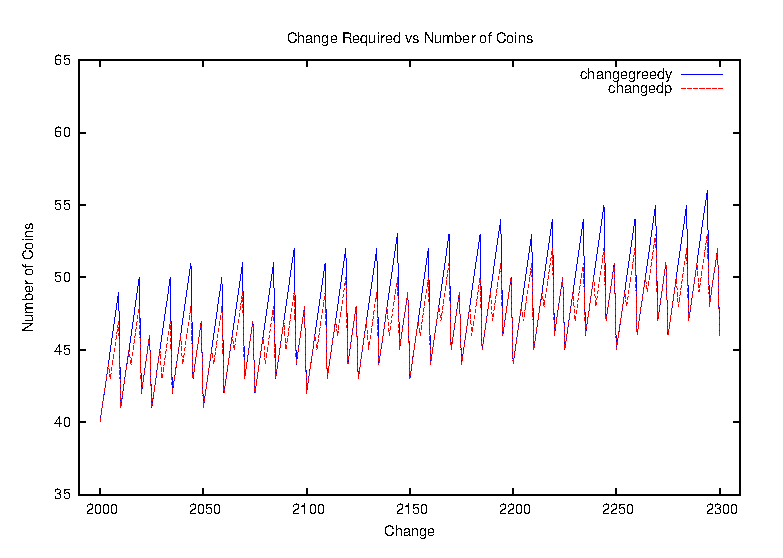
\includegraphics[width=\textwidth]{graph.eps}
There are times where both functions find the same number of coins, and there are time where the functions differ by at most 3. But they both have a similar increasing and decreasing slope over the same values of C.

\section{Experimental Runtime}
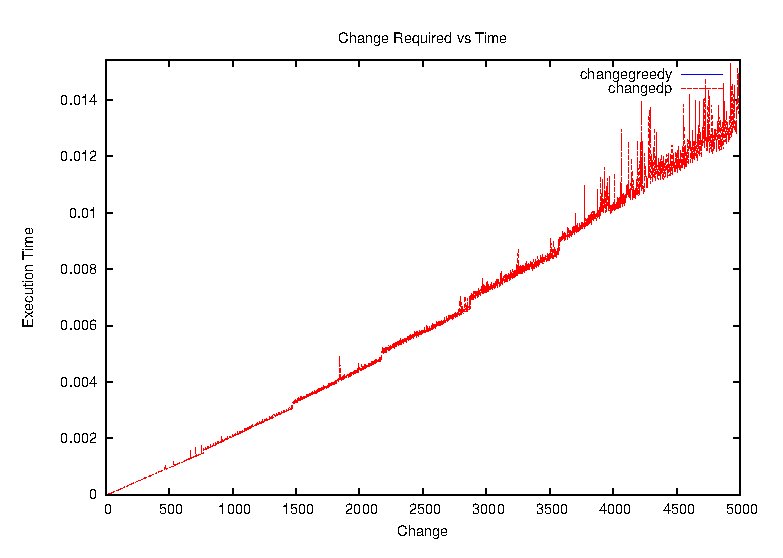
\includegraphics[width=\textwidth]{graph2-normal.eps}
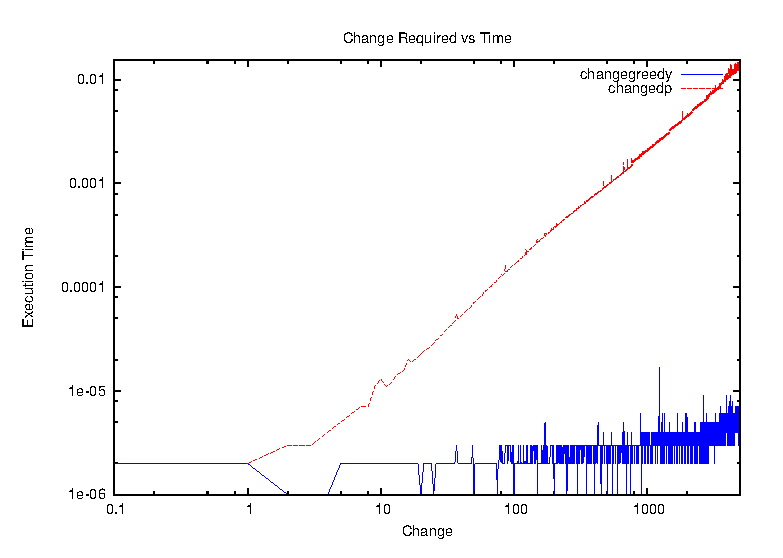
\includegraphics[width=\textwidth]{graph2-log.eps}

It appears that changedp has a linear slope on the loglog plot while changegreedy has a constant slope in the loglog plot.

Using 2 data points from the timing results in changedp (0.000011s, 9 and 0.015415s, 5000) and plugging them into the equation:
\begin{equation}\label{eq:Slope}
Slope = m = \frac{log(\frac{F_{1}}{F_{0}})}{log(\frac{x_{1}}{x_{0}})}
\end{equation}

results in $m = 1.1464$ which means that changedp is at least $O(n^{1.1464})$.\\

For changegreedy, the runtime goes from 0.000001s for change size 1 to 0.000007 for change size 5000. this means that changegreedy is roughly $cn$ with $c < 1$. This mean that the asymptotic runtime of our implementation of changegreedy is $O(n)$

\section{Coins Required for Values of C}
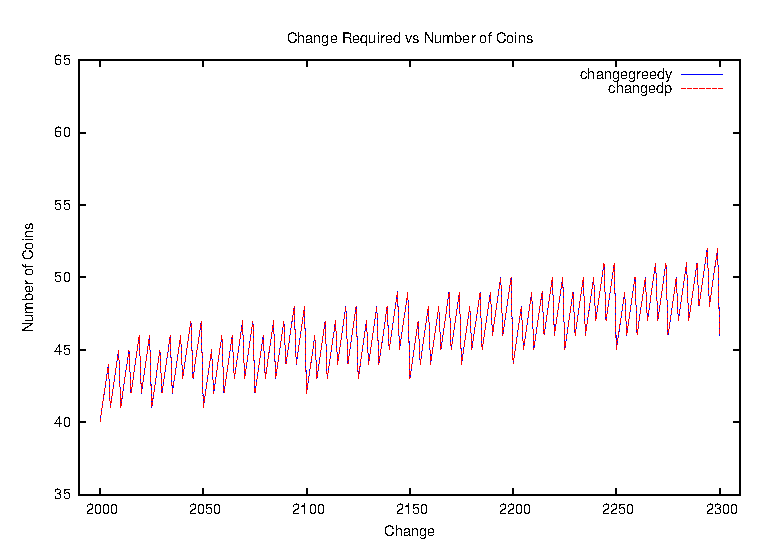
\includegraphics[width=\textwidth]{graph2.eps}

In this case, both approaches find the the same amount of coins to make change for each value.

\section{Coins as Values of P}

The only thing that would change in this example is the base for each coin that you would use to divide the amount into.

\section{Coins for which changegreedy fails but changedp does not?}

Yes. Let $V = [10, 25]$ and $C = 90$. Greedy would get stuck because it would use $3 25$ options, and $1 10$ option. This would leave $5$ left over, but no way to make change for it. The changedp however, would find $9 10$ and be able to make correct change.s

\end{document}
